\subsubsection{Materials}
Before trying FCT, the test participants played a small demo of the Camera Path Animator \cite{unity_camTool}. It uses the "Angry Bots" game provided by Unity \cite{angryBots} with a solider seen from above moving around a military facility.

Three scenes were constructed for the evaluation of FCT, each with gradually more complex geometry (see Figure \ref{fig:sceneAll}). 
The first scene consists of simple boxes of various shapes and colors. This was used to let the test participants try basic navigation in Unity.
The second scene is a simple sandbox-like environment with a pre-defined path. Small rocks have been added to make it easier to orientate oneself. The test participants were asked to complete tasks in this scene.
The third scene depicts a mountainous environment with a staircase attached to the mountainside, again with a pre-defined path. The scene's purpose is to let the test participants be creative and create their own framings. Contrary to the two previous scenes, this scene has variety in both height and depth. The intention is to allow for more creative freedom.

%The first was an environment with simple geometry scene. The second was used in the first part of the test when participants were introduced to the camera tool and had to complete 5 tasks. The third level was for the creative part of the test when participants had to envision the camera movement in an environment and then implement it. 

\begin{figure}[htbp]
\centering
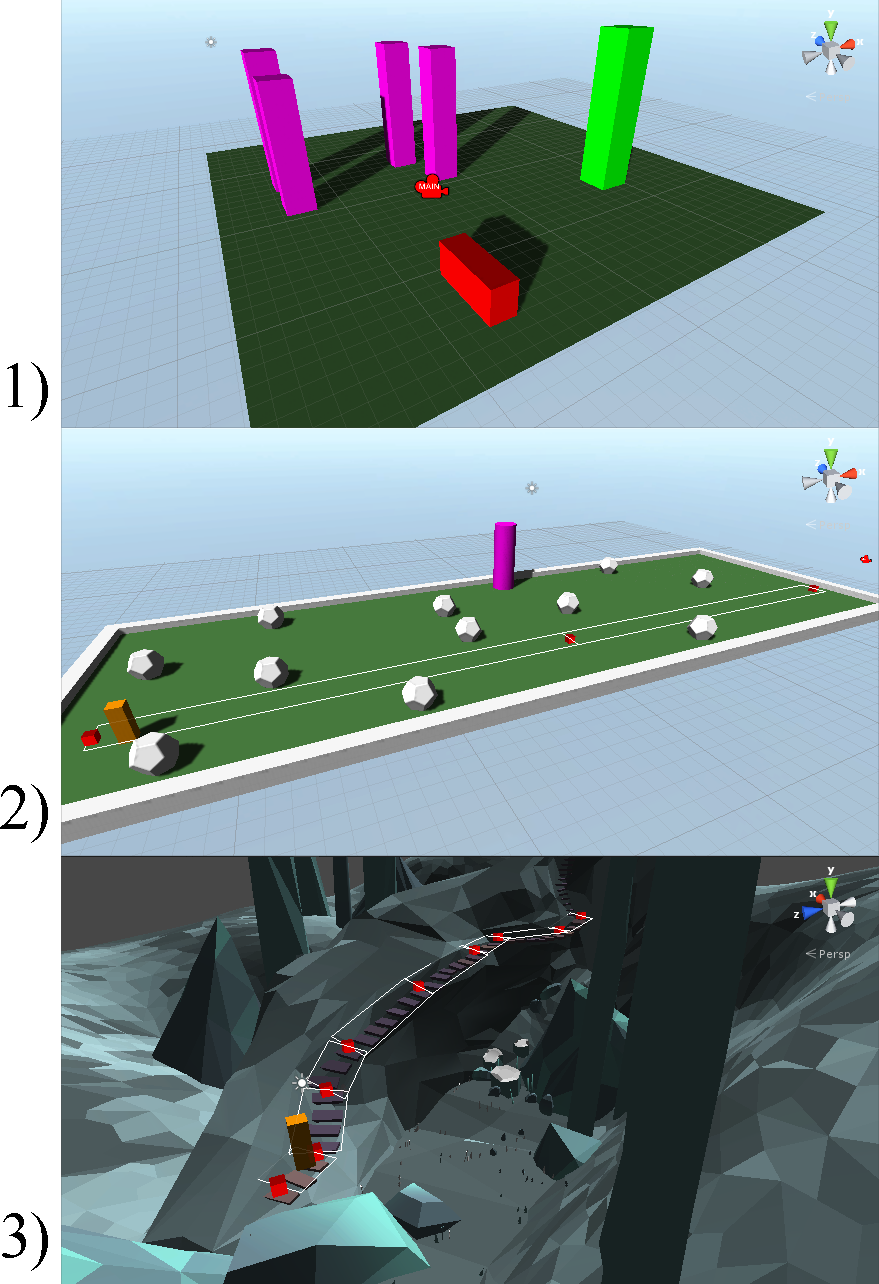
\includegraphics[width=0.3\textwidth]{Pics/sceneAll}
\caption{The evaluation consisted of three parts, each with their own scenes. The first scene is for getting a feel of basic navigation in Unity. The second scene is used for the test participants to try out the camera tool. The third scene is for the creative task where the test participants created their own framings.}
\label{fig:sceneAll}
\end{figure}